\subsection*{Определение основных операций в пространстве $\mathbb{R}^2$. }

\noindent \textbullet~Рассмотрим пространства $\mathbb{R}^2$. Зададим на него некоторые обозначения:

\smallskip
1) $(\overline{x}, \overline{y}) = x_1 y_1 + x_2 y_2$ - скалярное произведение векторов.

\smallskip
2) $\norm{\overline{x}} = \sqrt{x_1^2 + x_2^2} = \sqrt{(\overline{x}, \overline{x})}$ - длина вектора.

\smallskip
3) $\cos(\widehat{\overline{x}, \overline{y}}) = \dfrac{(\overline{x}, \overline{y})}{\norm{(\overline{x}, \overline{y})}}$. - косинус угла между векторами.

\smallskip
\noindent \textasteriskcentered~Ортогональные векторы - косинус между которыми равен $90^\circ$: 
$\overline{x} \bot \overline{y} \Longleftrightarrow \widehat{\overline{x}, \overline{y}} = 0$.

\medskip
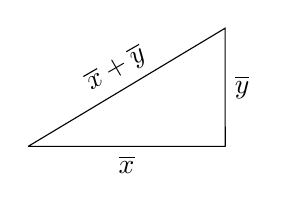
\begin{tikzpicture}[scale=0.5]

\draw (0, 0) -- (5, 0) -- (5, 3) -- node[rotate=30, above]{$\overline{x} + \overline{y}$} (0, 0);
\draw (2.5, 0) node[anchor=north] {$\overline{x}$};
\draw (5, 1.5) node[anchor=west] {$\overline{y}$};
\draw (5, 0) rectangle (5, 0.5);

\end{tikzpicture}

\medskip
\noindent \textbullet~$\norm{\overline{x}}^2 + \norm{\overline{y}}^2 = \norm{\overline{x} + \overline{y}}^2$. Проверим.

\smallskip 
\noindent \textbullet~$\norm{\overline{x} + \overline{y}}^2 = (\overline{x} + \overline{y}, \overline{x} + \overline{y})$. Из формулы для скалярного произведения 
очевидно, что $(\alpha\overline{x} + \beta \overline{y}, \overline{z}) = \alpha(\overline{x}, \overline{z}) + \beta (\overline{y}, \overline{z})$. Тогда согласно 
этому соотношению: $(\overline{x} + \overline{y}, \overline{x} + \overline{y}) = (\overline{x}, \overline{x}) + (\overline{x}, \overline{y}) +
(\overline{y}, \overline{x}) + (\overline{y}, \overline{y}) = (\overline{x}, \overline{x}) + (\overline{y}, \overline{y}) = \norm{\overline{x}}^2 +
\norm{\overline{y}}^2$.

\medskip 
\noindent \textbullet~Также рассмотрим сложение векторов по правилу параллелограмма:
$2\norm{\overline{x}}^2 + 2\norm{\overline{y}}^2 = \norm{\overline{x} + \overline{y}}^2 + \norm{\overline{x} - \overline{y}}^2$.

\medskip 
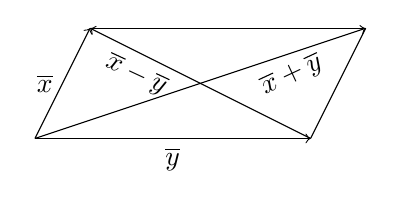
\begin{tikzpicture}[scale=0.7]
    \draw[->] (0, 0) -- node[anchor=east]{$\overline{x}$} (1, 2);
    \draw[->] (0, 0) -- node[anchor=north]{$\overline{y}$} (5, 0);
    \draw (1, 2) -- (6, 2);
    \draw (5, 0) -- (6, 2);
    \draw[->] (0, 0) -- node[anchor=north, near end, rotate=25]{$\overline{x} + \overline{y}$} (6, 2);
    \draw[->] (5, 0) -- node[anchor=north, near end, rotate=-25]{$\overline{x} - \overline{y}$} (1, 2);
\end{tikzpicture}

\medskip
\noindent \textbullet~Имея линейное многообразие $\mathbb{R}^2 = \{ \overline{x} = (x_1, x_2)\}$ сложение точек и умножение точки на число выполняется покомпонентно и 
выстраивая в этом линейном многообразии величину $(\overline{x}, \overline{y}) = x_1 x_2 + y_1 y_2$ и назвав ее скалярное произведение мы дальше чисто формально можем 
определить длину вектора $\norm{\overline{x}} = \sqrt{(\overline{x}, \overline{x})}$, понятие ортогональности
$\overline{x} \bot \overline{y} \Longleftrightarrow \widehat{\overline{x}, \overline{y}} = 0$ и используя эти вещи формально выводить такие вещи как т.~Пифагора и 
равенство параллелограмма. И причем по формуле скалярного произведения заметим, что эта величина линейна по первой переменной:
$(\alpha \overline{x} + \beta \overline{y}, \overline{z}) = \alpha (\overline{x}, \overline{z}) + \beta (\overline{y}, \overline{z})$ - билинейный функционал, а также 
выполняется соотношение $(\overline{x}, \overline{y}) = (\overline{y}, \overline{x})$ поскольку $x_1, x_2 \in \mathbb{R}$. Также при умножении вектора на себя 
$(\overline{x}, \overline{x}) \ge 0$, $= 0 \Longleftrightarrow \overline{x} = 0$.


\subsection*{Пространство $\mathbb{R}^n$. }

\noindent \textbullet~Теперь рассмотрим $n$-мерные пространства: $\mathbb{R}^n = \{ \overline{x} = (x_1, x_2, \dots, x_n), x_k \in \mathbb{R}\}$. Операция и умножение
на число переносятся точно также, скалярное умножение задается как $(\overline{x}, \overline{y}) = \sum_{k = 1}^n x_k y_k$, длина вектора $\norm{\overline{x}} = 
\sqrt{(\overline{x}, \overline{x})}$. Теорема Пифагора и равенство параллелограмма сохраняются, мы задавали их формально.


\subsection*{Бесконечномерные пространства. }

\noindent \textbullet~Также хочется рассматривать бесконечномерные векторы $\overline{x} = (x_1, x_2, \dots, x_n, \dots)$. Сложение поординатное и умножение на множитель
точно также. Если взять ту же формулу для скалярного произведения, то получается бесконечная сумма слагаемых (результат не определен). Остается только заузить линейное 
многообразие бесконечномерных векторов таким образом, чтобы в рамках бесконечномерного многообразия формула для скалярного произведения сохранилась. С этой целью 
рассмотрим пространство $l_2 = \{ \overline{x} = (x_1, x_2, \dots) : \sum_{k = 1}^\infty x_k^2 < +\infty \} $. 

\smallskip 
\noindent \textbullet~По неравенству Гельдера для $p = 2$ получается $\abs{\sum_1^\infty x_k y_k} \le \sum_1^\infty \abs{x_k} \abs{y_k} \le 
\sqrt{\sum_1^\infty x_k^2} \cdot \sqrt{\sum_1^\infty y_k^2} \Rightarrow \sum_1^\infty x_k y_k$ - конечное. Таким образом, в $l_2$ скалярное произведение определено 
по аналогии с пространством $\mathbb{R}^n$ : $(\overline{x}, \overline{y}) = \sum_1^\infty x_k y_k$, норма определеляется как $\sqrt{\sum_1^\infty x_k^2} = 
\sqrt{(\overline{x}, \overline{x})}$. $\mathbb{R}^2 \rightarrow \mathbb{R}^n \rightarrow l_2$. 


\subsection*{Бесконечномерные пространства в поле комплексных чисел. Унитарное пространство. }

\noindent \textbullet~Теперь распространим скалярное произведение на абстрактную ситуацию. Пришли к абстрактной конструкции: 1) рассматриваем в поле комплексных чисел 
$\mathbb{C} = \{ z = x + i y, x, y \in \mathbb{R}, i^2 = -1\}$. Операции сложения $z_1 + z_2$ и умножения $z_1 \cdot z_2$ определены по соответствующим формулам, 
символ $\overline{z} = x - i y$ - сопряженный элемент, модуль - $\abs{z} = \sqrt{x^2 + y^2}$ и он обладает свойством $\abs{z_1 + z_2} \le \abs{z_1} + \abs{z_2}$. Также 
непосредственно проверяется: $z \cdot \overline{z} = \abs{z}^2, \; \overline{z_1 z_2} = \overline{z_1} \cdot \overline{z_2}, \; \overline{z_1 + z_2} = 
\overline{z_1} + \overline{z_2}, \; \abs{\overline{z_1} \cdot \overline{z_2}} = \abs{\overline{z_1}} + \abs{\overline{z_2}}$.

\bigskip 
\noindent \textasteriskcentered~Пусть $X$ - линейное многообразие над $\mathbb{C}$, $x + y$, $\alpha x$, $\alpha \in \mathbb{C}$, 
а также определена величина $\varphi(x, y)$, удовлетворяющая следующим аксиомам:

\smallskip
1) $\varphi(x, x) \ge 0$, $= 0 \Longleftrightarrow x = 0$;

\smallskip
2) $\varphi(x, y) = \overline{\varphi(y, x)}$;

\smallskip
3) $\varphi(\alpha x + \beta y, z) = \alpha \varphi(x, z) + \beta \varphi(y, z)$ - линейность по первому аргументу

\smallskip 
\noindent тогда $\varphi$ - \textit{скалярное произведение} на $X$ и обозначается $\varphi(x, y) = (x, y)$.

\medskip 
Как пример, возьмем $X = l_2$ над $\mathbb{C}$, $\overline{x} \in l_2$, $\overline{x} = (x_1, x_2, \dots) : x_k \in C$, $\sum_1^\infty \abs{x_k}^2 < + \infty$ - модуль 
потому что комплексное число, а также определено скалярное произведение $(\overline{x}, \overline{y}) = \sum_{k = 1}^\infty x_k \overline{y}_k$. Все аксиомы проверяются 
непосредственно.

\smallskip
\noindent \textasteriskcentered~Тогда пара объектов $(X, (x, y))$ - \textit{унитарное пространство} модели $l_2$ над полем $\mathbb{C}$.

\medskip
\begin{theorem*}[неравенство Шварца]
Пусть $X$ - унитарное пространство. Тогда $\forall x, y \in X \Rightarrow \abs{(x, y)}^2 \le (x, x) \cdot (y, y)$.    
\end{theorem*}

\begin{proof}
\smallskip
\par\noindent \textbullet~$\forall \lambda \in \mathbb{C}$ и по первой аксоиме $(\lambda x + y, \lambda x + y) \ge 0$. Раскроем данное неравенство по аксиомам, учитывая 
следующие моменты: 1) $(\lambda x, y) = \lambda(x, y)$, 2) $(x, \lambda y) = \overline{(\lambda y, x)} = \overline{\lambda (y, x)} =
\overline{\lambda} \cdot \overline{(y, x)} = \overline{\lambda} \cdot (x, y)$, т.е множитель выносится с комплексным сопряжением со второй позиции, 3) $(x, y + z) = 
\overline{(y + z, x)} = \overline{(y, x) + (z, x)} = \overline{(y, x)} + \overline{(z, x)} = (x, y) + (x, z)$.

\smallskip
\noindent \textbullet~Таким образом, $(\lambda x + y, \lambda x + y) = (\lambda x, \lambda x + y) + (y, \lambda x + y) = (\lambda x, \lambda x) + (\lambda x, y) + 
(y, \lambda x) + (y, y) = \lambda \overline{\lambda} (x, x) + \lambda(x, y) + \overline{\lambda} (y, x) + (y, y) \ge 0 \; \forall \lambda \in \mathbb{C}$. В частности 
это неравенство выполнится, если $\lambda = - \dfrac{(y, x)}{(x, x)}$; $\overline{\lambda} = - \dfrac{\overline{(y, x)}}{(x, x)} = - \dfrac{(x, y)}{(x, x)}$. Подставим и 
посчитаем.

\[
    \left( - \dfrac{(y, x)}{(x, x)}\right) \cdot \left( - \dfrac{(x, y)}{(x, x)}\right) \cdot (x, x) - \left(\dfrac{(y, x)}{(x, x)}\right) \cdot (x, y) - 
    \left(\dfrac{(x, y)}{(x, x)}\right) \cdot (y, x) + (y, y) \ge 0
\]

\smallskip
\noindent \textbullet~Домножим на неотрицательный $(x, x)$ и сократим:

\[
    \abs{(x, y)}^2 - \abs{(x, y)}^2 - \abs{(x, y)}^2 + (x, x) \cdot (y, y) \ge 0 \Rightarrow \abs{(x,y)}^2 \le (x, x) \cdot (y, y)
\]
\end{proof}

\medskip
\noindent \textbf{Утверждение.} \textit{Функционал $\norm{x} = \sqrt{(x, x)}$ удовлетворяет всем 3-м аксиомам абстрактной нормы. }

\medskip
\begin{proof}
   
\noindent1)~$\norm{x} \ge 0$, $= 0 \Longleftrightarrow x = 0$ - очевидно;

\smallskip 
\noindent2)~$\norm{\alpha x} = \sqrt{(\alpha x, \alpha x)} = \sqrt{\abs{\alpha}^2 \cdot (x, x)} = \abs{\alpha} \cdot \sqrt{(x, x)} = \abs{\alpha} \cdot \norm{x}$;

\smallskip 
\noindent3)~По неравенству Шварца: $\norm{x + y}^2 = (x + y, x+ y) = (x, x) + (x, y) + (y, x) + (y, y) = \norm{x}^2 + (x, y) + (y, x) + \norm{y}^2 \le 
\norm{x}^2 + \abs{(x, y)} + \abs{(y, x)} + \norm{y}^2 \le \norm{x}^2 + 2 \norm{x} \norm{y} + \norm{y}^2 = (\norm{x} + \norm{y})^2$. Извлекаем корень и 
получаем неравенство: $\norm{x + y} \le \norm{x} + \norm{y}$.
\end{proof}

\medskip 
\noindent \textbullet~В любом унитарном пространстве $X$, $\norm{x} = \sqrt{(x, x)}$ определяет норму на $X$. Таким образом, унитарное пространство - частный случай 
общих нормированных пространств. Оно отличается тем, что в этом пространстве норма задается конкретной формулой через скалярное произведение. Поэтому все понятия, которые 
были раньше для нормированных пространств, они могут быть использованы и здесь.
